\section{Database Annotation Errors} \label{sec:Clustering_Anomalies}

To evaluate the anomalies in \autoref{fig:PCA_Cluster_Knee_4} \textbf{\textsf{B}} and \textbf{\textsf{C}}  an evolutionary distance were calculated by \gls{MSA} for every eventually misplaced sequence (\autoref{sec:MAFFT}). Therefore the eventually misplaced sequence was compared to a sample of 5 sequences from the same cluster related to the dominant subtype of the cluster, as well as to a sample of 5 sequences with subtype equal to the misplaced sequence but from other clusters. The mean of distances was then calculated for both cases to rate the assignment and reveal possible misannotations in the \gls{IRD}. 

\begin{table}[!hbt]
    \centering
    \caption[Anomalies in Segment 4 Cluster 2 (\Acrshort{PCA})]{\textbf{Anomalies in Segment 4 Cluster 2 (\Acrshort{PCA}).}.}
    \label{tab:PCA_Error_4_2}
    \pgfplotstabletypeset[
        every head row/.style={
            before row={
                \toprule
            },
            after row={
                \midrule
            },
        },
        every last row/.style={
            after row={
                %... & ... & ... & ... & ... & ... & ... & ...\\
                \bottomrule
            },
        },
        begin table=\begin{tabular*}{0.75\textwidth},
        end table=\end{tabular*},
        columns={0,1,2},
        columns/0/.style={string type,multicolumn names=l,column name=\textbf{Accession}, column type=@{\extracolsep{\fill}\hspace{6pt}}l},
        columns/1/.style={multicolumn names=l,column name=\textbf{H1}, column type=l},
        columns/2/.style={multicolumn names=l,column name=\textbf{H10}, column type=l},
    ]
    {PCA/error_segment_4_cluster_2_difference_head.csv}
\end{table}

In case of \autoref{fig:PCA_Cluster_Knee_4} \textbf{\textsf{C}} a single sequence with subtype H10 was classified as belonging to the cluster 2 which other than that completely consist of H1 and unclassified sequences. By investigation on this possible misplacement the mentioned comparison with \gls{MSA} was used. The results for this comparison in table \autoref{tab:PCA_Error_4_2} points to the fact, that the as H10 annotated sequence with accession MK237334 is related to subtype H1. The mean of evolutionary distance based on \glspl{MSA} is very low in comparison to a sample of cluster 0 H1 sequences especially when considering the size of cluster 0. The distance in comparison to a sample of random H10 sequences is much higher. Even when considering the random sampling on the different H10 cluster and the possible error by high differences between the sequences of the clusters, is a misannotation still more likely, since only this sole sequence of annotated as subtype H10 is present in a cluster of over 900 sequences of H1. 

\begin{table}[!hbt]
    \centering
    \caption[Anomalies in Segment 4 Cluster 48 (\Acrshort{PCA})]{\textbf{Anomalies in Segment 4 Cluster 48 (\Acrshort{PCA}).}.}
    \label{tab:PCA_Error_4_48}
    \pgfplotstabletypeset[
        every head row/.style={
            before row={
                \toprule
            },
            after row={
                \midrule
            },
        },
        every last row/.style={
            after row={
                ... & ... & ...\\
                \bottomrule
            },
        },
        begin table=\begin{tabular*}{0.75\textwidth},
        end table=\end{tabular*},
        columns={0,1,2},
        columns/0/.style={string type,multicolumn names=l,column name=\textbf{Accession}, column type=@{\extracolsep{\fill}\hspace{6pt}}l},
        columns/1/.style={multicolumn names=l,column name=\textbf{H16}, column type=l},
        columns/2/.style={multicolumn names=l,column name=\textbf{H13}, column type=l},
    ]
    {PCA/error_segment_4_cluster_48_difference_head.csv}
\end{table}

When comparing the distances for \autoref{fig:PCA_Cluster_Knee_4} \textbf{\textsf{C}} in \autoref{tab:PCA_Error_4_48} no decision for misannotation can be made. The dominant subtype in the cluster 48 is H16 but the sequences of subtype H13 that seem to be misplaced in the cluster have a smaller distance to the sample of sequences from subtype H13. The difference in distance to sample sequences of H13 as well as for sequences for H16 gave indeed no clear finding, since both results are quite similar and the misclustered sequences seem to share much sequence similarity with both subtypes. Therefore the sequences seem have more degrees of similarity than two represented by the known subtypes. Maybe the misclustered sequences in cluster 48 point to a more complex classification. Cluster 48 is a inconclusive cluster with many sequences from subytype H13 and H16 and therefore treated as clustering error. Subtype H13 and H16 are the focus of investigations of the clustering behaivior in the following sections to reveal possible subdivisions.

\begin{figure}[!hbt]
    \centering
    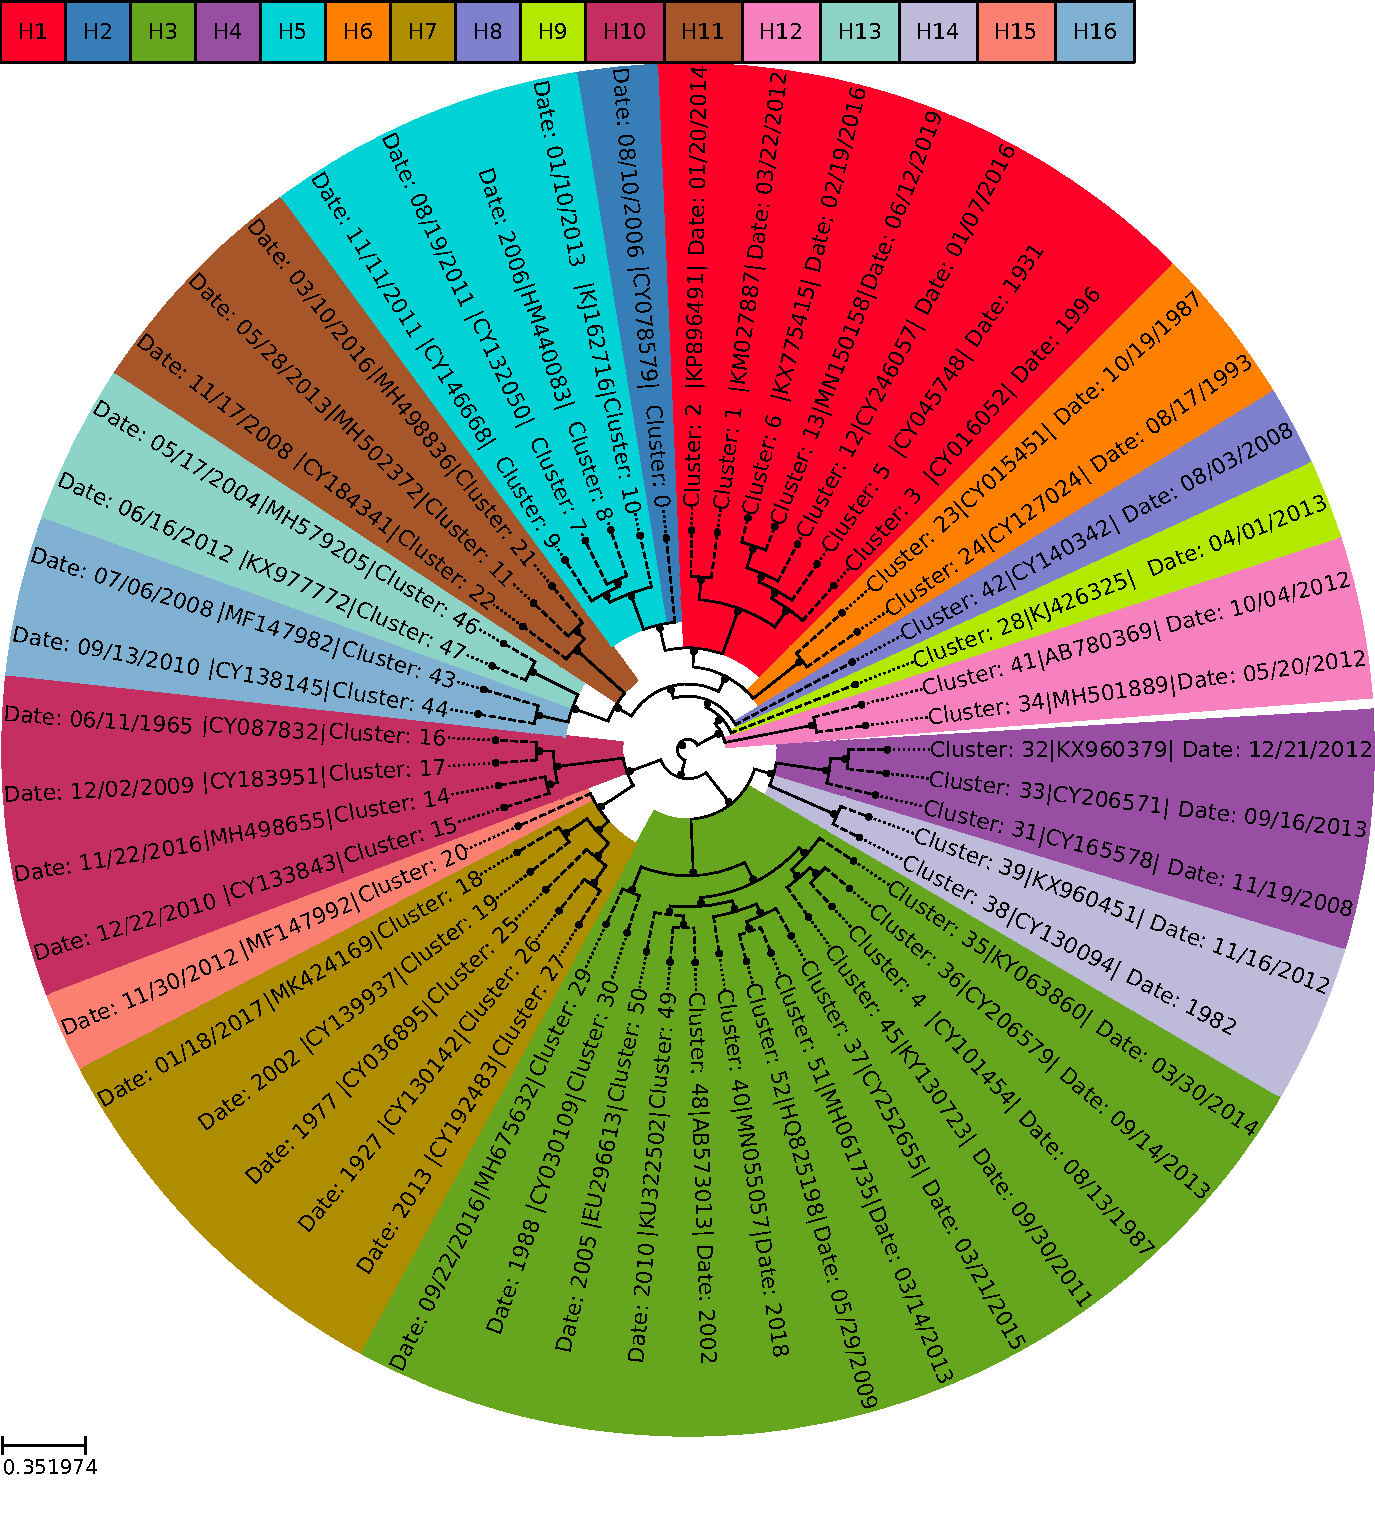
\includegraphics[width=\textwidth]{PCA/Guidetree_segment_4_H_Centroid.pdf}
    \caption[Knee based Segment 4 Centroid Guidetree (\Acrshort{PCA})]{\textbf{Knee based Segment 4 Centroid Guidetree (\Acrshort{PCA}).} .}
    \label{fig:PCA_Guidetree_Centroid_4}
\end{figure}

The anomalie involving cluster 4 that is split off the other clusters homogeneous for H3 sequences \autoref{fig:PCA_Cluster_Knee_4} \textbf{\textsf{D}} is evaluated by comparison to a guide-tree from the centroid sequences. Every of the 55 clusters have a sequence that should represent the whole cluster, the centroid sequence, calculated as described in \autoref{sec:MAFFT}. By building an alignment over these 55 centroid sequences a guide-tree was created (\autoref{fig:PCA_Guidetree_Centroid_4}). When using the guide-tree as comparison the uniform color distribution stand out. Even cluster 4 is arranged in a line with all cluster homogeneous for subtype H3. Therefore cluster 4 and 48 (\autoref{fig:PCA_Cluster_Knee_4} \textbf{\textsf{C}} and \textbf{\textsf{D}}) are treated as clustering mistakes and are further examined in the following.

%Übergang zu cluster Comparison durch Centroid Alignment Tree -> H13/H16 Clustertree, Alignmenttree Vergleich -> Cluster H13/H16 Comparison
%fehler im clustering oder fehler in der DAtenbank